\documentclass{article}
\usepackage[polish]{babel}
\usepackage[OT4]{fontenc}
\usepackage[utf8]{inputenc}
\usepackage{hyperref}
\usepackage{graphicx}
\usepackage{float}
\usepackage{amsmath}
\usepackage{indentfirst}

\title{\textbf{Praca projektowa z przedmiotu Sztuczna Inteligencja}}
\author{Bartłomiej Czajka 169522 2 EF-DI P1}
\date{Rzeszów, 2023}
\linespread{1.5}
\begin{document}
\maketitle
\pagebreak



\tableofcontents{}
\section{Opis projektu}
\subsection{Założenia projektowe}
Celem projektu jest realizacja sieci neuronowej uczonej za pomocą algorytmu sieci głębokiej, klasyfikującej chorobę Parkinsona oraz zbadanie wpływu parametrów sieci na proces uczenia.
Projekt został zrealizowany w języku Python z wykorzystaniem biblioteki PyTorch.
\subsection{Zestaw danych}
Zestaw danych uczących został pobrany ze strony \href{http://archive.ics.uci.edu/ml/datasets/Parkinsons}{http://archive.ics.uci.edu/ml/datasets/Parkinsons}.
Zawiera on 197 instancji, 23 cechy oraz 2 klasy. Dane są nieuporządkowane, nie ma danych nieokreślonych.
Dokładniejszy opis cech zestawu:
\begin{itemize}
    \item name - Nazwa badanego pacjenta w ASCII i numer nagrania.
    \item MDVP:Fo(Hz) - Średnia częstotliwość podstawowa głosu.
    \item MDVP:Fhi(Hz) - Maksymalna częstotliwość podstawowa głosu.
    \item MDVP:Flo(Hz) - Minimalna częstotliwość podstawowa głosu.
    \item MDVP:Jitter(\%), MDVP:Jitter(Abs), MDVP:RAP, MDVP:PPQ, Jitter:DDP - Kilka miar zmienności częstotliwości podstawowej.
    \item MDVP:Shimmer, MDVP:Shimmer(dB), Shimmer:APQ3, Shimmer:APQ5, MDVP:APQ, Shimmer:DDA - Kilka miar zmienności amplitudy.
    \item NHR, HNR - Dwie miary stosunku szumu do składowych tonalnych w głosie.
    \item status - Stan zdrowia badanego (jeden) - chory na Parkinsona, (zero) - zdrowy.
    \item RPDE, D2 - Dwie miary złożoności dynamicznej nieliniowej.
    \item DFA - Wykładnik skalowania fraktalnego sygnału.
    \item spread1, spread2, PPE - Trzy nieliniowe miary zmienności częstotliwości podstawowej.
\end{itemize}
\subsection{Przygotowanie danych}
Sieć ma za zadanie sklasyfikować czy pacjent cierpi na chorobę Parkinsona. Wartość '1' oznacza osobę cierpiącą na chorobę Parkinsona, natomiast '0' oznacza osobę zdrową.
Dane zostały uporządkowane i znormalizowane.
Normalizacja została wykonana dla każdej obserwacji przy użyciu wzoru:
\[
    x_{\text{norm}} = \frac{{x_{\text{norm\_max}} - x_{\text{norm\_min}}}}{{x_{\text{max}} - x_{\text{min}}}} \cdot (x - x_{\text{min}}) + x_{\text{norm\_min}}
\]

gdzie:
\begin{itemize}
    \item $x_{min}$ - to wektor zawierający minimalne wartości dla każdej obserwacji.
    \item $x_{max}$ - to wektor zawierający maksymalne wartości dla każdej obserwacji.
    \item $x_{norm\_min}$ - to wartość minimalna po normalizacji (-1).
    \item $x_{norm\_max}$ - to wartość maksymalna po normalizacji (1).
    \item $x_{norm}$ - to macierz zawierająca znormalizowane dane.
    \item $x$ - to macierz zawierająca dane wejściowe.
\end{itemize}
\section{Zagadnienia teoretyczne}
\subsection{Matematyczny opis sztucznego neuronu}
Podstawowym elementem budującym strukturę sieci neuronowej jest neuron. Jest to element, który przetwarza informacje.
W pewnym, uproszczonym stopniu jest wzorowany na funkcjonowaniu biologicznej komórki nerwowej.
Struktura neuronu zawiera wiele wejść oraz jedno wyjście.
Jednym z najważniejszych składników neuronu są wagi, których wartości decydują o zachowaniu neuronu. Są one zazwyczaj ustalane w trakcie procesu uczenia.
\begin{figure}[H]
    \centering
    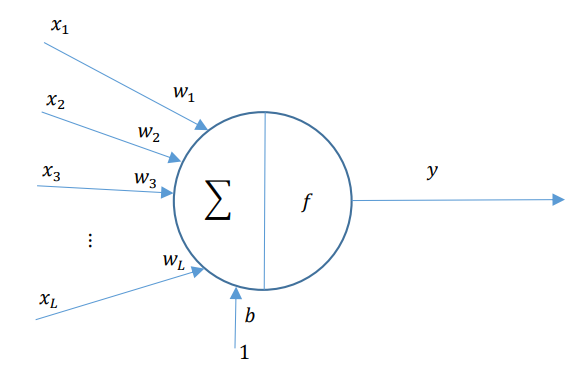
\includegraphics[width=0.8\textwidth, keepaspectratio]{model_neuronu.png}
    \caption{Model neuronu [4]}
    \label{fig:zdjecie}
\end{figure}

Każdy pojedynczy neuron przyjmuje sygnały wejściowe, które są następnie przetwarzane.
Każde wejście ma przypisany współczynnik wagowy, który określa jak bardzo wpływa ono na wynik neuronu.
Dodatkowo, neuron posiada "bias", czyli dodatkowe wejście, na którym występuje stała wartość.
Wszystkie te informacje są sumowane, gdzie jest obliczane łączne pobudzenie neuronu.
Następnie wartość pobudzenia przechodzi przez funkcję aktywacji, która określa sygnał wyjściowy neuronu dany wzorem:
\[
    y = \sum_{j=1}^{L} f(w_{j} x_{j} + b)
\]

gdzie:
\begin{itemize}
    \item $j$ -- indeks, który przyjmuje wartości od 1 do $L$,
    \item $y$ -- wyjście neuronu,
    \item $w_{j}$ -- współczynnik wagowy przypisany do $j$-tego wejścia,
    \item $x_{j}$ -- $j$-ty sygnał wejściowy,
    \item $b$ -- bias [2].
\end{itemize}

\subsection{Funkcja aktywacji}
Sam model matematyczny neuronu nie byłby wystarczający do skomplikowanych obliczeń w m.in. sieciach głębokich.
Należy wprowadzić funkcje aktywacji, które nadają sieciom neuronowym zdolność modelowania nieliniowych relacji między danymi wejściowymi, a wyjściowymi.
Dzięki tej nieliniowej transformacji na wyjściu sztucznego neuronu, możliwe jest wprowadzenie nieliniowości i bardziej skomlipowanych obliczeń.
Istnieje wiele funkcji aktywacji.

Szczególnie przydatną w modelach głębokich ze względu na swoją prostotę i skuteczność jest funkcja ReLU, która została przeze mnie wykorzystana jako funkcja aktywacji dla warstw ukrytych.
Działa na zasadzie przekazywania wartości dodatnich bez ich zmiany, natomiast dla wartości ujemnych przypisuje zerową wartość.
Matematycznie można zdefiniować ją następującym wzorem:
\[
    f(x) = \max(0, x)
\]
Innymi słowy, funkcja ReLU jest zdefiniowana na przedziale:
\[
    f(x) = \begin{cases}
        0, & \text{gdy } x \leq 0, \\
        x, & \text{gdy } x > 0.
    \end{cases}
\]
gdzie:
\begin{itemize}
    \item $x$ -- wartość wejściowa na której zostanie zastosowana funkcja aktywacji.
\end{itemize}

Istnieje również funkcja aktywacji softmax, która dla danego wektora wyników \( \mathbf{z} = (z_1, z_2, \ldots, z_n) \) gdzie \( n \) oznacza liczbę klas, funkcja softmax przekształca każdy element \( z_i \) na wartość prawdopodobieństwa \( p_i \).
Funkcję softmax można zdefiniować w następujący sposób:


\subsection{Sieć głęboka}
Sieci głębokie to rodzaj modeli uczenia maszynowego, które składają się z wielu warstw neuronów, zwanych warstwami głębokimi.
Każda warstwa wykonuje operacje na danych wejściowych, a następnie przekazuje wyniki do kolejnej warstwy, aż do warstwy wyjściowej, która generuje ostateczne predykcje lub wyniki.

Warstwa sieci głębokiej składa się z macierzy wag (w), wektora przesunięć (b), funkcji aktywacji (f) oraz wektora sygnałów na wyjściu warstwy (y).

\begin{figure}[H]
    \centering
    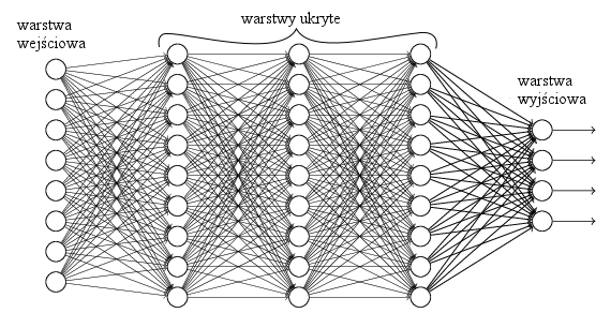
\includegraphics[width=1\textwidth, keepaspectratio]{siec_gleboka.png}
    \caption{Sieć głęboka [5]}
    \label{fig:siec}
\end{figure}



\section{Realizacja sieci neuronowej}
\subsection{Opis skryptu}
\section{Eksperymenty}
\subsection{Eksperyment 1}
\subsection{Eksperyment 2}
\subsection{Eksperyment 3}
\section{Wnioski}
\begin{thebibliography}{9}
    \bibitem{Nielsen}
    Michael Nielsen,
    \emph{Neural Networks and Deep Learning}.
    Determination Press,
    2015.
    \bibitem{TadeusiewiczSzaleniec}
    Ryszard Tadeusiewicz, Maciej Szaleniec,
    \emph{Leksykon sieci neuronowych}.
    Wrocław,
    2015.
    \bibitem{vandeput}
    Nicolas Vandeput,
    \href{https://medium.com/analytics-vidhya/a-brief-history-of-neural-networks-c234639a43f1}{\emph{A Brief History Of Neural Networks}},
    [dostęp: 17.05.2023].
    \bibitem{zajdel}
    Zajdel R.,
    \emph{Ćwiczenie 4 Model Neuronu},
    Rzeszów,
    KIiA, PRz.
    \bibitem{gora}
    Paweł Gora,
    \href{https://www.deltami.edu.pl/temat/informatyka/sztuczna_inteligencja/2017/12/28/Glebokie_uczenie_maszyn/}{\emph{Głębokie uczenie maszyn}},
    [dostęp: 17.05.2023].
    \bibitem{zajdel}
    Zajdel R.,
    \emph{Procedura przygotowania danych dla sieci neuronowych na potrzeby projektu z modułu sztuczna inteligencja - Listing1},
    Rzeszów,
    KIiA, PRz.
    \bibitem{zajdel}
    Zajdel R.,
    \emph{Procedura przygotowania danych dla sieci neuronowych na potrzeby projektu z modułu sztuczna inteligencja - Listing2},
    Rzeszów,
    KIiA, PRz.
\end{thebibliography}
\end{document}